\chapter{基于本体的地理知识问答系统}\label{chapter:al_sup}
基于本体的地理知识问答是指根据构建的地理本体知识库,构建一个基于知识库的问答系统,针对用户提出的地理问题给出精准的答案。本章首先介绍本文的系统任务分析和系统总体设计,然后介绍系统详细设计,最后介绍系统实现环境。

\section{系统任务分析}
本论文任务是:根据用户提出的地理问题,系统直接给出该问题的简短、精准答案。如下为用户所提出的四个问题和系统相应回复答案举例:

(1)提问:“地球的半径大约是多少呢?”,回复:“6371km”

(2)提问:“地球半径约多少米多少千米?”,回复:“6371km”

(3)提问:“怎样保护热带雨林?”,回复:“加强环境教育,提高公民环保意识;加强雨林管理和保护,建立自然保护区。”

(4)提问:“中国采取了哪些措施保护热带雨林?”,回复:“加强环境教育,提高公民环保意识;加强雨林管理和保护,建立自然保护区。”

问题(1)、(2)问的为同一个问题,均可根据本文知识库中三元组“(地球,半径,6371km)”来回答。问题(3)、(4)也是问的相同问题、只是语言不同,均可根据知识库中三元组“(雨林,保护措施内容,“加强环境教育,提高公民环保意识;加强雨林管理和保护,建立自然保护区”)”来回答,系统需要区分知识库中“雨林”和问题中问的“热带雨林”其实为同一个概念。因此,本文主要有两个任务,如下:

(1)构建可以回答地理问题的地理本体知识库。

(2)在构建的地理本体知识库上构建问答系统,系统需满足用户按不同语言组织方式随意提问,均能正确匹配知识库中可以回答问题的答案三元组。

\section{系统总体设计}
针对基于本体的地理知识问答的两个任务,即本体知识库的构建任务和基于注意力机制的地理知识库问答任务,本文设计了如下图\ref{fig:graduation}所示的系统总体结构图。

\begin{figure}[!htb]
	\centering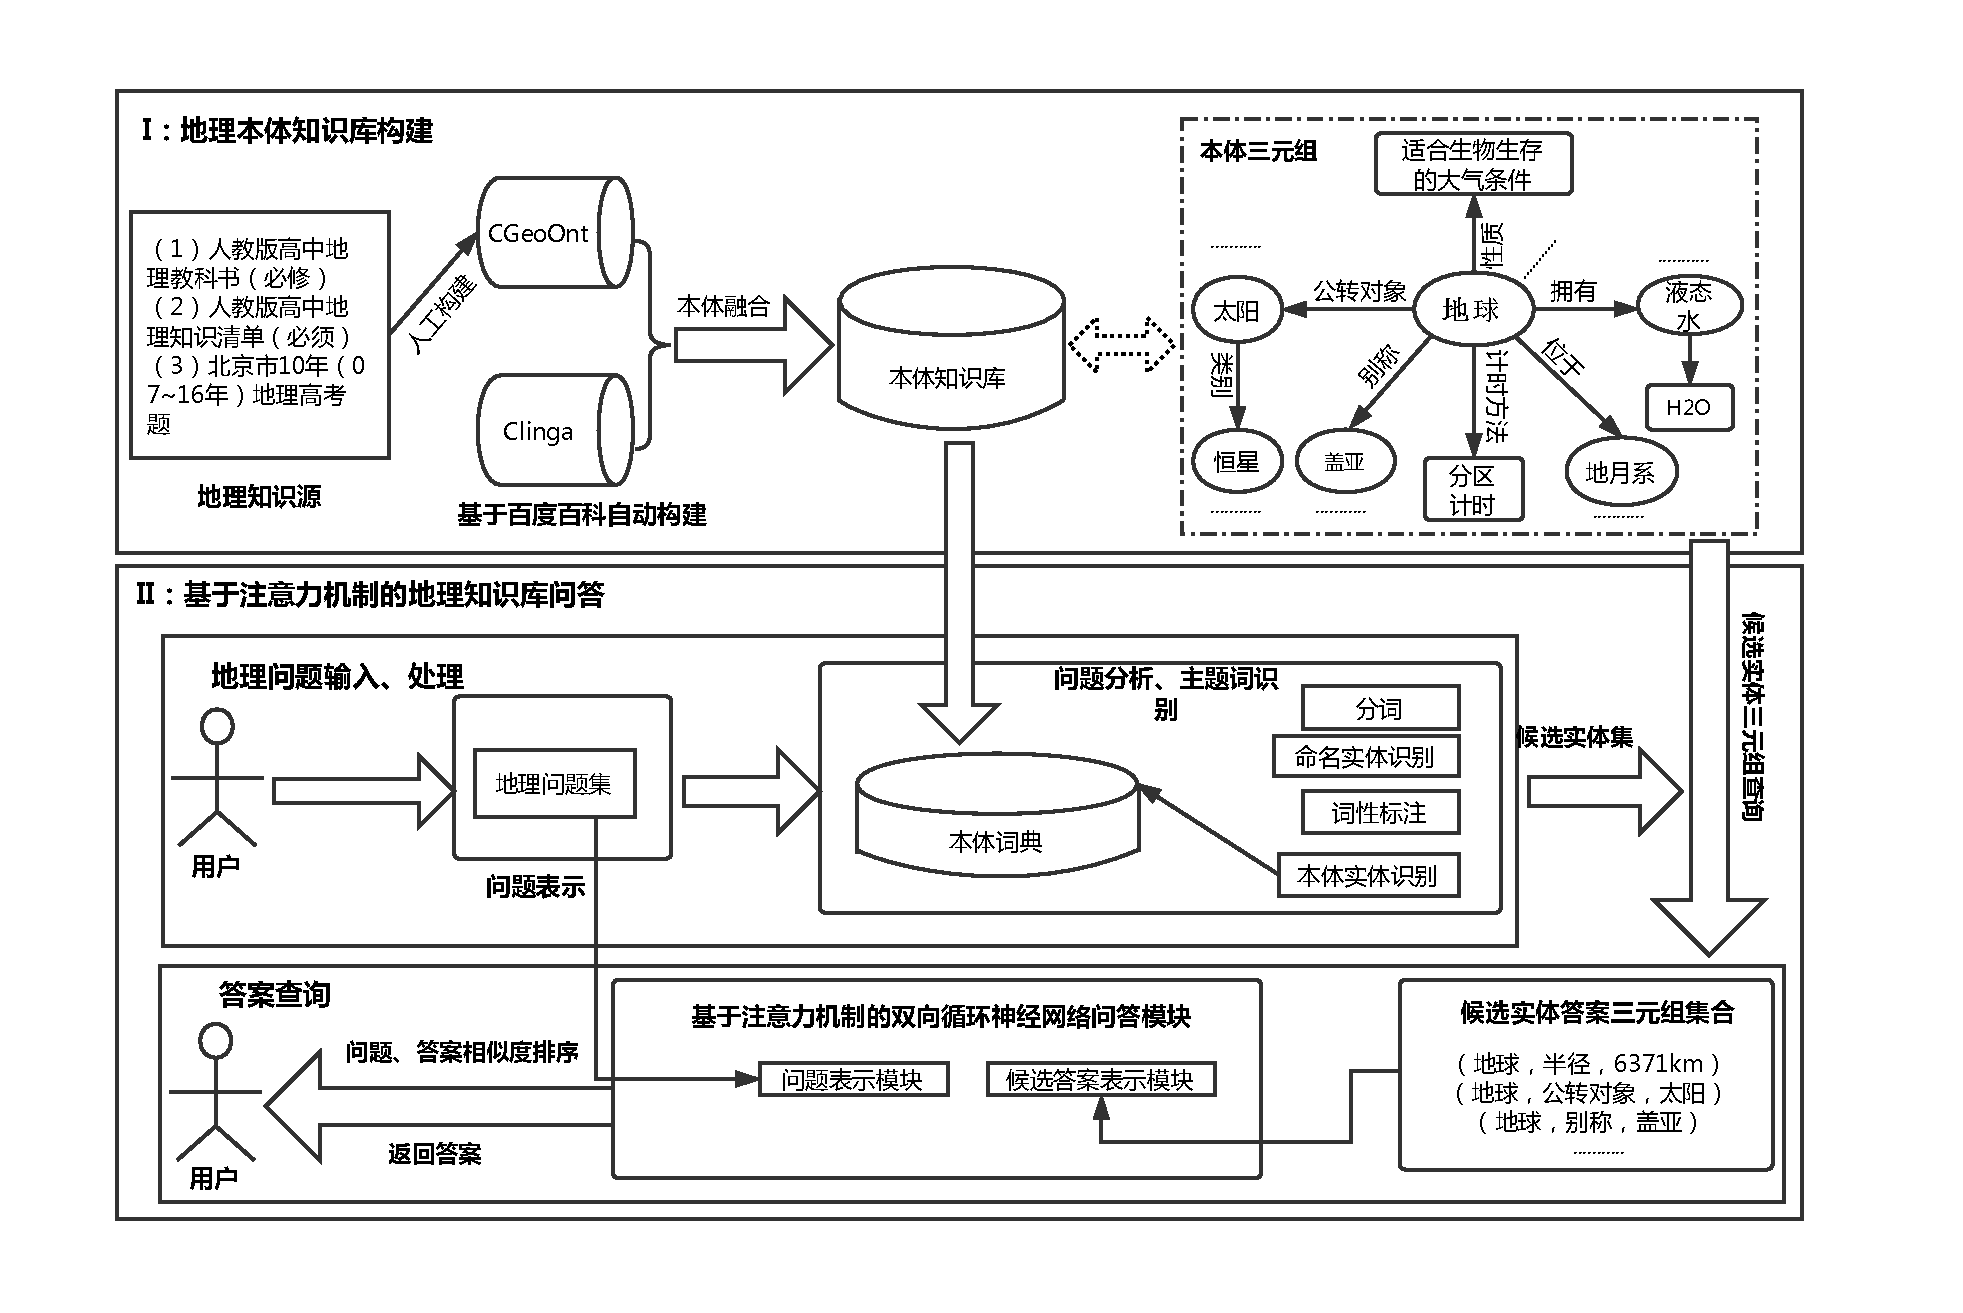
\includegraphics[height=9cm]{resource/graduation}
	\caption{基于本体的地理知识问答系统结构图}
	\label{fig:graduation}
\end{figure}

\subsection{功能模块结构设计}
该系统总体结构图由两个模块组成,地理本体知识库构建模块、基于注意力机制的地理知识库问答模块。第二个模块包括两个子模块:地理问题输入、处理模块和答案查询模块

地理本体知识库构建模块包括三个任务,第一是根据高中地理相关知识源人工构建地理本体CGeoOnt,第二是将本体CGeoOnt和基于百度百科自动构建的地理本体Clinga融合成更大的本体并进行本体存储和检索,第三个任务是根据融合而成的地理本体构建本体词汇表和本体同义词词汇表,本文统称为为本体词典。

基于注意力机制的地理知识库问答模块的子模块——地理问题输入、处理模块包括两个任务,第一是根据地理核心知识考点,获取跟知识考点相关的真实地理问题集,第二是对问题进行分析,包括问题分词、命名实体识别、词性标注和问题中包含的本体主题词识别,最终目的是生成候选答案实体供候选答案检索。

基于注意力机制的地理知识库问答模块的子模块——答案查询模块包括三个任务,第一是根据候选答案实体去地理本体知识库查询相应的候选答案三元组,第二是构建地理知识库问答模型对用户输入的问题和其候选答案进行向量表示,第三是根据问题和候选答案的向量表示,由相似度打分策略和最终答案选择策略选取最终答案。

\subsection{总体工作流程设计}
该系统问答流程如图\ref{fig:qa_overview}所示,图\ref{fig:qa_overview}表示的是地理问题“2016年北京处暑节气是什么时间”被回答的流程。首先,需要识别该地理问题中的主题实体,也就是问题是围绕哪个实体概念在提问的,如此问题中考察的是“北京的处暑节气时间”,是考察跟“北京”相关的事实性知识,因此“北京”为主题实体。然后,根据主题实体“北京”从本文构建的知识库中查询出与“北京”直接相连的所有实体作为候选实体,此处为首尔和华盛顿等。最后使用双向循环神经网络对此问题和候选答案三元组——北京、首尔、华盛顿的三元组进行词向量表示,取问题与候选答案三元组相似度最大的三元组作为该问题的答案。

总结本文知识库问答任务,可分为如下四步进行:

\begin{figure}[!htb]
	\centering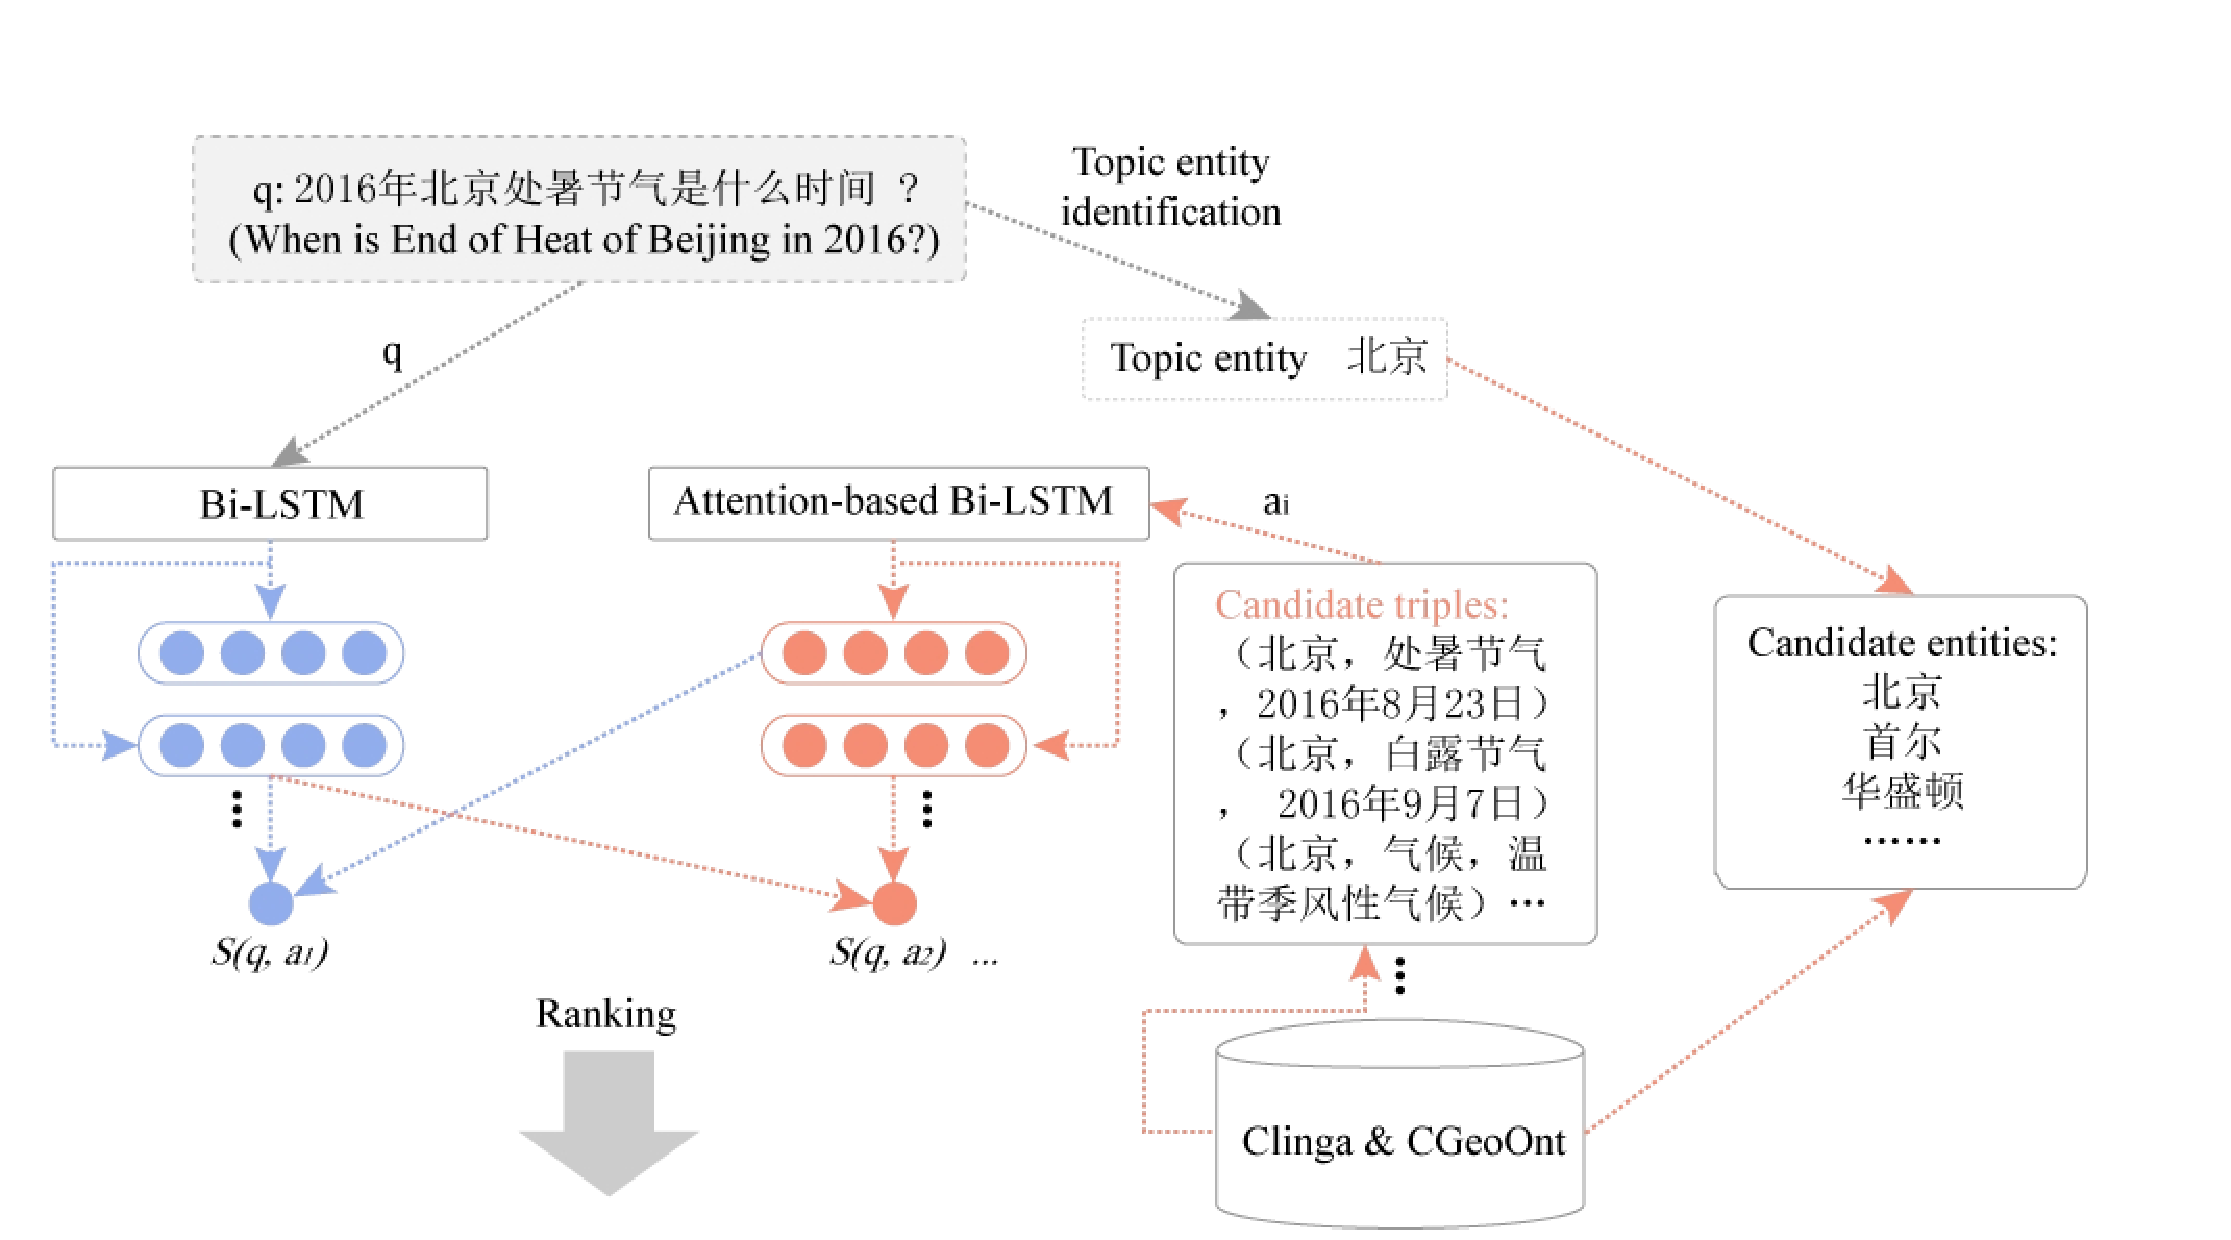
\includegraphics[height=7cm]{resource/qa_overview_1}
	\caption{基于注意力机制的地理知识库问答流程}
	\label{fig:qa_overview}
\end{figure}

( 1)识别地理问题中涉及的主题实体,根据主题实体生成候选实体集。

(2)根据候选实体集查询知识库,返回候选实体三元组。

( 3)使用双向 LSTM 神经网络编码问题(问题词序列表示成词向量),使用基于注意力机制的双向 LSTM编码候选答案三元组。

( 4)计算问题与每个候选答案三元组的余弦相似度值,返回余弦值最大的三元组作为最终答案(有时返回多个最终答案, 详见 3.3.4)。


\section{系统详细设计}
系统详细设计分别对本文问答系统的两个模块进行叙述,这两个模块分别是地理本体知识库构建模块和基于注意力机制的地理知识库问答模块。地理本体知识库构建模块的叙述见第四章,基于注意力机制的地理知识库问答模块包括候选实体答案三元组生成、基于注意力机制的地理知识库问答模型和问题最终答案选取策略三部分。
\subsection{地理本体知识库构建}
地理本体知识库构建的叙述见第四章

\subsection{候选实体答案三元组生成}
生成候选实体答案三元组需要识别问题中的主题实体,主题实体应当存在于本文所构建的知识库中,如果知识库中不存在此主题实体,则问题回答失败。

本文根据知识库构建实体概念词典以及实体概念别名词典,确定知识库能够回答的实体问题范围。候选答案实体三元组生成的关键是识别出问题中的主题实体,如下(1)-(3)为主题实体识别流程,(4)-(5)步为根据主题实体生成候选答案实体三元组:

(1)使用分词工具jieba\footnote{https://pypi.org/project/jieba/}将问题进行分词,生成问题的词序列。

(2)对词序列进行命名实体识别(Named Entity Recognition, NER)、词性标注(Part  of  Speech, POS), 识别其中的命名实体、名词以及名词词组,本文称为候选主题实体集。

(3)遍历(2)步中生成的候选主题实体集,查询该候选实体是否在本文本体词典中,若存在,则该实体视作主题实体;若为本体词典中词的子串(不包含相等的情况),亦将该实体视作主题实体;若所有候选主题实体都不存在于本体词典中,则此问题没有主题实体,此题目超出本文知识库的回答范围,回答失败。

(4)从本文地理知识库中获取跟主题实体一跳1-hop和二跳2-hop的实体集合作为候选答案实体集。

(5)最后,从知识库查询出候选答案实体集每个实体的三元组信息,构成目标候选答案实体三元组集合。

\subsection{基于注意力机制的地理知识库问答模型}
基于注意力机制的地理知识库问答模型的叙述见第五章。

\subsection{问题最终答案选取策略}
在测试阶段,问答模型给所有候选答案打分排序,选择出得分最高的答案三元组$S_{max}$,考虑到一个问题的正确答案可能不止一种,因此,本文设置答案阈值,此阈值取损失函数中的m,将得分与最高分相差不超过m的三元组也视作最终答案。如下:$C_q$为问题q的所有候选答案集合,$\widehat{A}_q$为最终答案集合,$\hat{a}$为候选答案。
$$
\mathcal{S}_{max} = \arg\max_{a \in C_q}{S(q,a)}
\eqno(1)
$$
$$
\widehat{A}_q = \{\hat{a}|S_{max} - S(q, \hat{a}) < m\}
\eqno(2)
$$

\section{系统实现环境}
本文地理知识库问答系统实验是在微软云服务器(Microsoft  Azure)上进行,具体硬件、软件环境如下所示:

硬件环境:

CPU: 4 $\times$ Intel(R) Xeon(R) CPU E5-2600 0 @ 2.20GHz

Memory: 14GB

软件环境:

系统:Ubuntu 16.04.4 LTS

编程语言:Python3.6.5 |Anconda

深度学习框架:Tensorflow 1.6.0

Python编辑器:VIM -Vi IMproved 7.4 \& Jupyter Notebook

知识库存储数据库:Virtuoso 7.2.4 Released

\section{本章小结}
本章介绍了基于本体的地理知识问答系统的具体实现过程。主要包括对本文两个主要任务——地理本体知识库构建和基于注意力机制的地理知识库问答实现过程进行详细阐述。本章首先介绍本文的任务分析和本文的系统总体设计图;然后介绍系统的详细设计,包括地理本体知识库构建,候选实体答案三元组生成、基于注意力机制的地理知识库问答模型和问题最终答案选取策略;最后介绍系统的实现环境,包括实验的硬件、软件环境。
